\chapter{Design Concepts}
\label{chap:design}
In this chapter we discuss some design decisions of LDBN such as
reasons for moving to a web-based application, platform choice and 
design ideas which were considered but not included in the final version. In the following the
term client is used to refer to a browser.

\section{Choice of Platform}
Due to the fact that web-enabled educational 
systems are becoming the dominant type of systems 
available to students, we designed LDBN as a web-based application.
In addition to this, web-based systems offer several advantages in comparison to 
standalone systems. They minimize the problems of distributing software to users 
and hardware and software compatibility. New releases of systems are immediately
available to everyone. More importantly, students are not
constrained to use specific machines in their schools, and can access 
web-based applications from any location and at any time. This type of independence 
is of enormous value for learning environments due to the importance of
flexibility and accessibility for the learning process.
 
The main issue, which really lies within the choice of platform, is the fact that there are
many different techniques for implementing a web-based application. A basic HTML-based
solution would not work since all pages in that case would be static. The remaining 
options can be divided into three groups:

\begin{enumerate}
	\item Client-side based
	\item Server-side based
	\item Client-server based
\end{enumerate}

The client-side solution consists of an application which runs entirely on the user's 
computer within a browser. Examples here could be the Java Applet, the Adobe Flash or the new 
Microsoft Silverlight technologies. However, this approach has the disadvantage
of requiring a plug-in, which is not always available by default on all web browsers. 
In addition, some organizations only allow software installed by the administrators. 
As a result, many users cannot view neither Java applets nor Adobe Flash by default. This could 
have a negative impact on the accessibility of an application; 
therefore we did not proceed with the client-side approach.

In the server-side solution there is a web server and optionally a data service. 
Web servers such as Apache, Tomcat, Lighttpd and IIS host the application 
logic, which is written in Java, PHP, Ruby, C\# or other languages. 
Data services are provided by databases systems such as MySQL, Oracle, SQL Server and 
so forth. This approach has a centralized architecture; thus all tasks and 
functions are performed on the server. After their completion a new HTML page is 
sent back to the client. This approach has two major drawbacks. In the first place, 
the browser must re-render the whole HTML page after each interaction with the server.
Although part of this could be avoided with the help of frames, it would still 
require more data than actually needed to be sent back to the client, since most 
parts of the page remain the same after each interaction. In the second place, 
all of the computations must be done on the server-side, leaving the client with 
the only task of rendering a page. This may result in a poor allocation of computational tasks. 
With the introduction of rich web-applications such as Google Maps, Facebook, 
Google Docs and others it has been shown in practice that the client is capable of 
much more than simply rendering a web page. 

Finally, there are client-server-based solutions, such as those
which use packages such as AJAX, which could be
seen as a mixture 
of the first two solutions. As it is used by LDBN, we
discuss AJAX more formally in the following section.

\section{AJAX}
\label{sec:ajax}
AJAX stands for Asynchronous JavaScript And XML. It should be noted
that AJAX is not a new technology in itself but rather the integration of several 
existing technologies, including HTML, CSS and JavaScript~\cite{w3}. Prior to AJAX browsers 
were treated 
like dumb terminals; thus the browser was unable to remember its state and every 
user interaction caused a HTTP round trip over the network, requiring browsers 
to re-render the whole web page after each request. With AJAX browsers became 
more powerful. Traditional web techniques like HTML and CSS are still used to 
render the page. In spite of that, JavaScript can be used to access 
and manipulate the Document Object Model (DOM) tree, i.e., 
JavaScript is capable of changing only certain parts
of the content of a web page. However, the
real potential of AJAX lies within the client-server communication, an example
of which is illustrated in Figure~\ref{fig:ajax01}. In this example we have an AJAX application
which runs within a browser. JavaScript must be enabled in the browser, otherwise
the application will not start.  
The XMLHttpRequest is an application programming interface (API) implemented by the browser,
which can be accessed by the application using JavaScript. This API is 
used to handle communication with the server in an asynchronous fashion using a
simple HTTP connection. It is worth mentioning that other solutions also exist. 
For example, XML is often used to transfer data between the server and the client, 
although XML is not required for data interchange and often other text-based
formats are used as an alternative such as JSON or plain text~\cite{bajax1}. In our example we have 
a web server which is used to establish a connection between the AJAX application and
the DBMS, where we store the data.

\begin{figure}[h]
	\begin{center}
		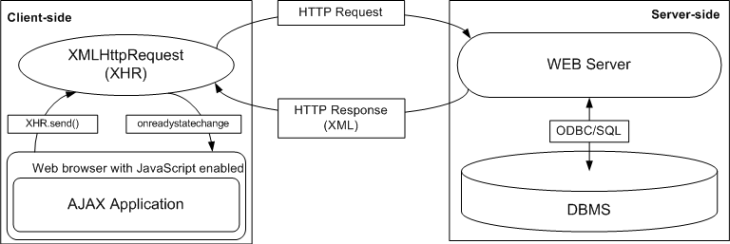
\includegraphics[width=0.8\textwidth]{./img/ajax01a.png}
		\caption{Example of an AJAX Architecture}
		\label{fig:ajax01}
	\end{center}
\end{figure}

Another advantage of AJAX is the so called \textit{Architectural Shift}~\cite{wgdd1}, 
which is illustrated in Figure~\ref{fig:ajax02}, which is
an adaptation of~\cite[Figure 3]{wgdd1}. 
It describes the ability of the client to handle events
locally, without the need of a server. Such events can be for example the
expansion of a tree. This has two advantages. On the one hand, it frees server 
and network resources for other tasks, on the other hand, it allows
the UI to be more interactive and to respond more quickly to inputs.

\begin{figure}[h]
	\begin{center}
		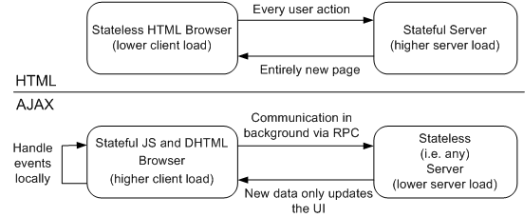
\includegraphics[width=0.8\textwidth]{./img/ajax02a.png}
		\caption{AJAX Architectural Shift}
		\label{fig:ajax02}
	\end{center}
\end{figure}

AJAX has also several shortcomings,
the biggest of which is the fact that it is not a standard. This has led to slight 
differences in the JavaScript language between browsers, along with major differences 
in the DOM and in the XMLHttpRequest API~\cite{bgwt1, bgwt2, bgwt3}. 
For our learning environment we need to support every major browser to ensure accessibility. 
However, this often requires writing a different code base for different browsers,
and this means less scalability for the application and less productivity 
for the developers~\cite{bgwt2}. Another major
disadvantage is the lack of good developer tools for JavaScript~\cite{bgwt2}, which also 
has a negative impact on the scalability and productivity.
A typical example here could be the debugging process of an AJAX project - 
often bugs are caused by a simple typographical error (typo), which in the case 
of JavaScript means that such errors can be found only at run time, and usually 
by end users~\cite{wgdd1}. 
These and other problems related with AJAX
led to the decision to use GWT - Google Web Toolkit~\cite{wgwt}, an introduction 
to which can be found in the following section.

\section{GWT} 
\label{sec:gwt}
Google Web Toolkit (GWT) is a set of tools and libraries that allows
web developers to create AJAX applications in Java~\cite{wgwt}. 
The tools are focused on solving the problem of moving the desktop application into the
browser~\cite{bgwt2}. GWT is an open source project and it is developed 
by Google. The major components of GWT include: 

\begin{enumerate}
	\item Java-to-JavaScript Compiler.
	\item Hosted Web Browser.
	\item JRE emulation library.
	\item Web UI class library.
	\item Many other libraries and APIs.
\end{enumerate}

The most important component is the Java-to-JavaScript compiler. It enables the 
translation of Java code into highly optimized, browser 
independent\footnote{As of GWT version 1.5, GWT supports: 
Firefox 1,~2,~3; Internet Explorer 6,~7; Safari 2,~3; Opera~9}
JavaScript code. 
In addition to this, it provides developers with compile-time error checking. 
Another very important
aspect of the compiler is the fact that when the code is compiled into JavaScript,
it results in 
a single JavaScript file for each browser type and target locale. This is illustrated 
in Figure~\ref{fig:gwt01}, which is an adaptation of~\cite[Figure 7]{wgio2}. 
Typically this means that a GWT application will be compiled into 
a minimum of five separate JavaScript files. Each of these files is meant to run 
on a specific browser type, version, and locale. A bootstrap script, initially 
loaded by the browser, will 
automatically pull the correct file when the
application is loaded. The benefit of this is that the code loaded by the browser 
will not contain code that it cannot use. The JavaScript code produced by the GWT 
compiler is highly optimized and it usually runs much faster than handwritten 
JavaScript code~\cite{wgio1}. Moreover, the development team must support only
one code base, by which the the scalability of an application can be increased.  

\begin{figure}[h]
	\begin{center}
		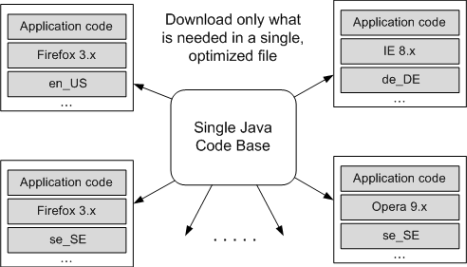
\includegraphics[width=0.8\textwidth]{./img/gwt01a.png}
		\caption{GWT Java-to-JavaScript Compiler}
		\label{fig:gwt01}
	\end{center}
\end{figure}

Another very important component is the hosted web browser. A GWT application can 
be run in hosted mode, this means 
the Java code is not compiled into JavaScript code but rather it is executed natively  
in a special hosted web browser. This browser works like any other web
browser, but it is specifically tailored for GWT development. It allows the developer
to make changes to the Java code and immediately see the results, without the need
of recompiling the source code. Furthermore, the hosted mode allows the use of 
very powerful development tools such as the Java debugger with all its functionality 
including placing a breakpoint. As Bruce Johnson~\cite{wgdd1}, 
the creator of GWT, has stated, before GWT this was nearly an impossible task in 
AJAX applications. With GWT developers can take full advantage of 
already existing development tools such as such as the Eclipse IDE~\cite{weclipse}. 
This can further increase the scalability of an application and the productivity 
of developers. 
In the case of LDBN, GWT helped scale the project to such extent that LDBN runs 
almost entirely on the client-side. In addition, LDBN has grown fast to 
more than 60 classes/interfaces. Debugging such large application without the powerful 
tools provided by GWT and Eclipse would have been nearly an impossible task for 
a single developer.

Other important components of GWT, which were also used in the development 
process of LDBN, include:

\begin{description}
	\item[JRE emulation library] This library contains 
	the most commonly used parts of the full Java Runtime Environment (JRE), 
	which can be compiled into JavaScript. LDBN uses extensively many of the collection 
	classes of the emulated library such as the \verb=ArrayList=, \verb=HashMap=, 
	and others classes.
	\item[Web UI library] GWT includes a large set of UI classes, which 
	enable the development of a web UI entirely in Java. The approach is similar 
	to writing a Java Swing application, and it is used to develop the whole UI 
	of LDBN. 
	\item[DOM API] GWT provides an abstraction on top of the DOM, 
	allowing the use of a single Java API without having to worry about 
	differences in implementations across browsers.
	\item[XML Parser] To make it as simple as possible to deal with XML data formats 
	on the client browser, GWT provides a DOM based XML parser.
	\item[RequestBuilder API] GWT also provides an abstraction on top of the
	XMLHttpRequest object. 
	\item[GWT-RPC] The GWT-RPC mechanism allows Java objects to be sent between 
	the client and the server. However, this is only true for 
	servlet containers such as the Apache Tomcat web server. 
	\item[JSNI] The JavaScript Native Interface (JSNI) makes it possible to
	write native JavaScript code within the Java code. The JavaScript code can 
	then be executed from Java code and vice versa - Java code can be executed
	from JavaScript code. JSNI is very important part of GWT, as it enables 
	the integration with already existing JavaSctipt applications.  
	\item[Internationalization] Several techniques are provided by GWT that can 
	aid with internationalization issues.
	\item[JUnit Integration] GWT provides support for JUnit~\cite{wjunit}, 
	a framework for making automated tests.
\end{description}

For additional literature on the subject of GWT, we recommend the book of 
Ryan Dewsbury \textit{Google Web Toolkit Applications}~\cite{bgwt2}. It has
proven to be very useful information source throughout the development process 
of LDBN.  

\section{Limitations of GWT and JavaScript}
Despite the fact that GWT offers solution to many of the problems
described in Section~\ref{sec:ajax}, it still has to deal with some 
fundamental issues regarding 
AJAX. Although the client-side application is written in Java, 
the code produced by the GWT compiler is still JavaScript, and
as such it has the following limitations:
   
\begin{enumerate}
	\item Single-thread environment.
	\item Same origin policy.
	\item No database connectivity.
\end{enumerate}

There is no way around the single-thread-environment issue. This can cause the UI
to become unusable for a while. In order to provide a more appropriate behavior 
for the UI, LDBN locks the entire UI before every extensive computation; e.g.,
testing the correctness of an assignment. When the UI is locked,
it gets dimmed and an image is indicating that the program is working. After 
completion the UI returns to its normal state. 

The same origin policy prevents AJAX applications from being used across domains,
although the W3C has a draft that would enable this functionality~\cite{bajax1}.

A browser-independent AJAX application is not capable of making a connection 
to a database~\cite{bajax1}, thus it requires a web server to establish the 
connection. Then the client-side communicate with the server-side using 
predefined XML format.

\section{Server-side Platform Choice}
In this section we give our reasons for choosing PHP as the server-side
scripting language and MySQL as the database management system (DBMS). First we would
like to mention that LDBN is open source and it is distributed under the 
Apache License, Version 2.0~\cite{walv2}. Furthermore, we would like to see 
LDBN installed on other servers as well. This could help LDBN become
a leading learning environment across 
different universities for teaching relational-database normalization. To ensure 
portability we have decided to use the most common free 
tools for web development. Apache Web Server with PHP and MySQL meet those requirements. 
Apache is the most popular HTTP server on the Web~\cite{w3} and PHP is the most popular 
Apache module~\cite{w4}. In addition, MySQL is the most popular open source 
database system~\cite{w5}.
 
It is worth mentioning that even though LDBN is implemented using Apache Web Server,
PHP and MySQL, it is possible to use different tools and programming languages 
on the server-side with almost no modifications to the client-side. However, 
the predefined XML data exchange format must stay the same.

\section{Other Design Issues}
An initial design of LDBN included an assignment generator, i.e., assignments were not
created by users, but rather automatically generated. However, this approach
has proven to be highly ineffective in terms of creating good assignments. There 
are many reasons for this, but the main one is the fact that it is not clear how
to determine good assignments. Every assignment could emphasize on different aspects of
the relational-database normalization, thus this approach has been disregarded.

